\documentclass[10pt]{article}

\usepackage[letterpaper,margin=0.45in,top=0.45in,bottom=0.55in,columnsep=0.15in]{geometry}
\usepackage{amsmath,amssymb}
\usepackage{graphicx}
\usepackage{microtype}
\usepackage{enumitem}
\usepackage{xurl}
\usepackage[hidelinks]{hyperref}
\usepackage{titlesec}
\usepackage[font=small,labelfont=bf,skip=4pt]{caption}
\usepackage{stfloats}
\usepackage{fancyhdr}
\pagestyle{fancy}
\fancyhf{}
\renewcommand{\headrulewidth}{0pt}
\fancyfoot[C]{\footnotesize\thepage}
\fancyfoot[L]{\footnotesize\itshape Do not distribute without written consent.}

\titleformat{\section}{\normalfont\large\bfseries}{\thesection}{0.6em}{}
\titleformat{\subsection}{\normalfont\normalsize\bfseries}{\thesubsection}{0.6em}{}
\titlespacing*{\section}{0pt}{1.0ex plus 0.3ex minus 0.2ex}{0.4ex}
\titlespacing*{\subsection}{0pt}{0.8ex plus 0.3ex minus 0.2ex}{0.3ex}
\setlength{\parskip}{0pt}
\linespread{0.95}
\setlength{\parindent}{1.2em}
\urlstyle{same}
\renewcommand{\dbltopfraction}{0.95}
\renewcommand{\textfraction}{0.05}
\renewcommand{\dblfloatpagefraction}{0.85}
\setcounter{dbltopnumber}{3}
\setlist[itemize]{leftmargin=1.2em,itemsep=1pt,topsep=2pt,parsep=0pt}

\graphicspath{{../artifacts/}}

\title{Epistemic Collapse in Multi-Agent Systems}
\author{Helivan \quad Calcifer Computing}
\date{}

\begin{document}
\makeatletter
\twocolumn[
  \begingroup
    \@maketitle
    \vspace{-1.75em}
    \centering
    {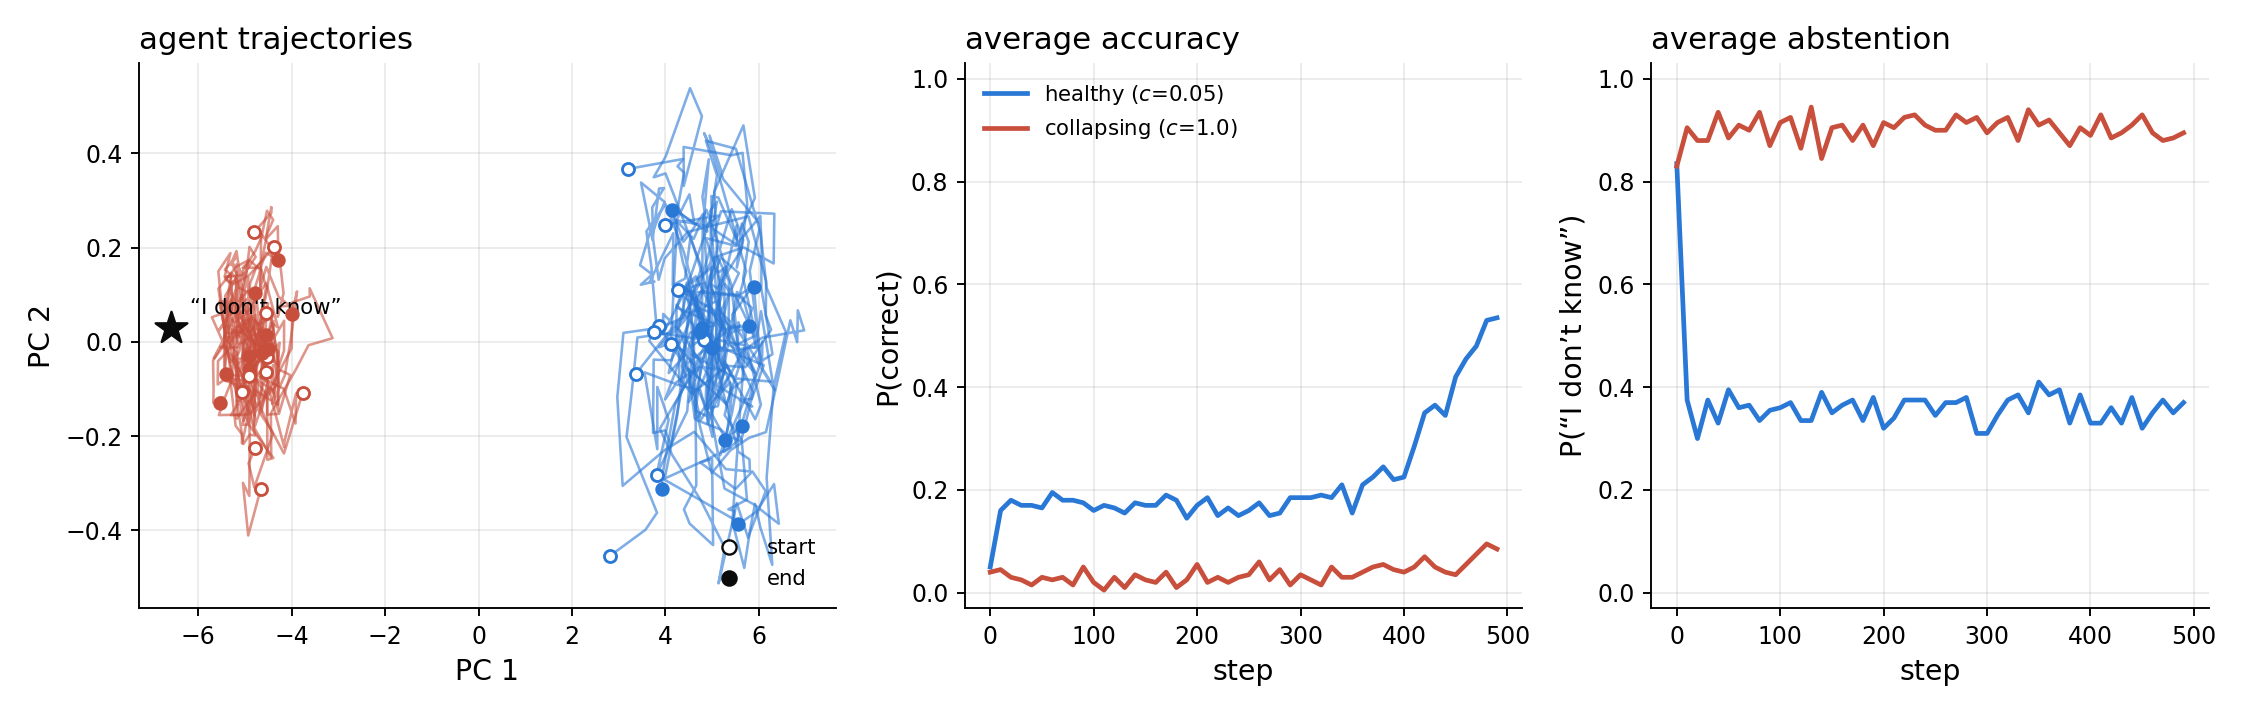
\includegraphics[width=0.93\textwidth]{fig_collapse_example.png}}
    \captionof{figure}{\textbf{A real multi-agent system experiencing epistemic collapse} (red), vs.\ a healthy control differing only in memory decay (blue; $c=1.0$ vs.\ $0.05$); $N=10$ gpt-4o-mini agents each. Left: agent trajectories in perspective space (each agent = its mean probe-response embedding per snapshot, smoothed; PCA over both runs; open = start, filled = end). The collapsing system's agents sit pinned to the ``I don't know'' point ($\star$) while healthy agents occupy the content-bearing region. Middle/right: average accuracy and average abstention over time. Setting described in Sec.~2.}
    \label{fig:example}
    \vspace{1.2em}
  \endgroup
]
\makeatother

\section{Motivation}
Information is being produced at unprecedented rates, and increasingly it is produced, relayed, and consumed by generative agents rather than people. An agent embedded in such a flow faces a compounding problem: whatever it has learned is decaying in relevance while new information arrives fast enough to crowd out the old. Communication is the standard remedy --- agents ask each other, repeat each other, and increasingly write to shared artifacts --- but communication moves evidence around; it does not keep evidence current. Our goal is to understand the \emph{benefits and limits of communication in a high-speed environment}: when does talking to peers, or maintaining a shared record, actually keep a population of agents knowledgeable, and when does it merely keep them \emph{confident}? Building on our earlier work on monitoring multi-agent systems (\emph{Control Charts for Multi-agent Systems}, arXiv:2605.11135), we study these questions in a real network of LLM agents and in a mechanistically faithful simulator, organized around a failure mode we call \emph{epistemic collapse}.

\section{Setting}
A system of $N=10$ gpt-4o-mini agents evolves for $T=500$ steps. Its components, by factor:

\textbf{Environment.} An external store holds the current true answer to each of $M=50$ questions (drawn from Natural Questions). No agent knows any truth except by consulting the environment. Every question is temporal: question $q$ is revised at rate $\lambda_q$ per step, with revisions appending a counter to the answer so that stale copies are detectably wrong. Speeds are heterogeneous across questions: $\lambda_q$ is log-normal with mean $\bar\lambda$ and dispersion 1, so a typical world mixes questions an order of magnitude faster and slower than $\bar\lambda$.

\textbf{Agents.} Each agent holds an unbounded memory of question--answer pairs, each tagged with its insertion time and provenance (firsthand observation vs.\ received). Retrieval for question $q$ returns the top $k_{\mathrm{ctx}}=3$ entries by relevance $\langle q,k\rangle\, e^{-c\,\mathrm{age}}$ on the insertion clock: old entries are never deleted, they are \emph{crowded out} by newer insertions, so forgetting is activity-dependent --- a busy agent forgets faster. The decay rate $c$ is the agent-side lever. Answering is done by the LLM from the retrieved context, under instruction to abstain (``I don't know,'' IDK) without grounding. Under the \emph{verbatim relay} protocol an agent may emit only an answer that originated in the environment, or IDK --- no paraphrase, so relayed content does not drift.

\textbf{Communication.} Agents sit on a fixed graph of specified mean degree. A peer ask targets a question the asker currently lacks, drawn uniformly; the peer's reply (possibly IDK) inserts into the asker's memory as received evidence. Each agent is seeded with 5 of the 50 questions at $t=0$.

\textbf{Observation.} Each agent spends exactly $B=11$ actions per step, split as $E$ environment queries and $K = B - E$ peer asks. An environment query returns the current truth, exact and freshly stamped. Observation is the only action that \emph{creates} current evidence; everything else redistributes it.

\textbf{Measurement.} On a fixed 20-question probe panel, averaged over the final 100 steps, we track four quantities: agent-level P(IDK) and P(correct) (mean over members) and system-level P(IDK) (no member answers) and P(correct) (some member is correct). These nest --- system IDK $\le$ agent IDK, agent correct $\le$ system correct --- so both levels share an axis.

\textbf{A measured surrogate.} Real runs cost money; most of our experiments run on a simulator with \emph{zero fitted parameters}. Under verbatim relay the LLM's causal role reduces to a gate --- given retrieved context, emit the stored payload or abstain --- and that gate is measurable: probing gpt-4o-mini across the (finitely many, up to exchangeability and similarity bucketing) context states yields a step function (target present $\Rightarrow$ answer w.p.\ $\approx0.95$--$1$; absent $\Rightarrow$ IDK w.p.\ $\approx0.95$--$1$; parametric leakage $\approx0$). Replacing the LLM call with this measured table reproduces the real system across all cells of the no-mimesis factor grid and the mimesis grid of Sec.~\ref{sec:mimesis} with median $|\Delta| = 0.01$ on all four metrics (Fig.~\ref{fig:cal}).

\begin{figure*}[b]
  \centering
  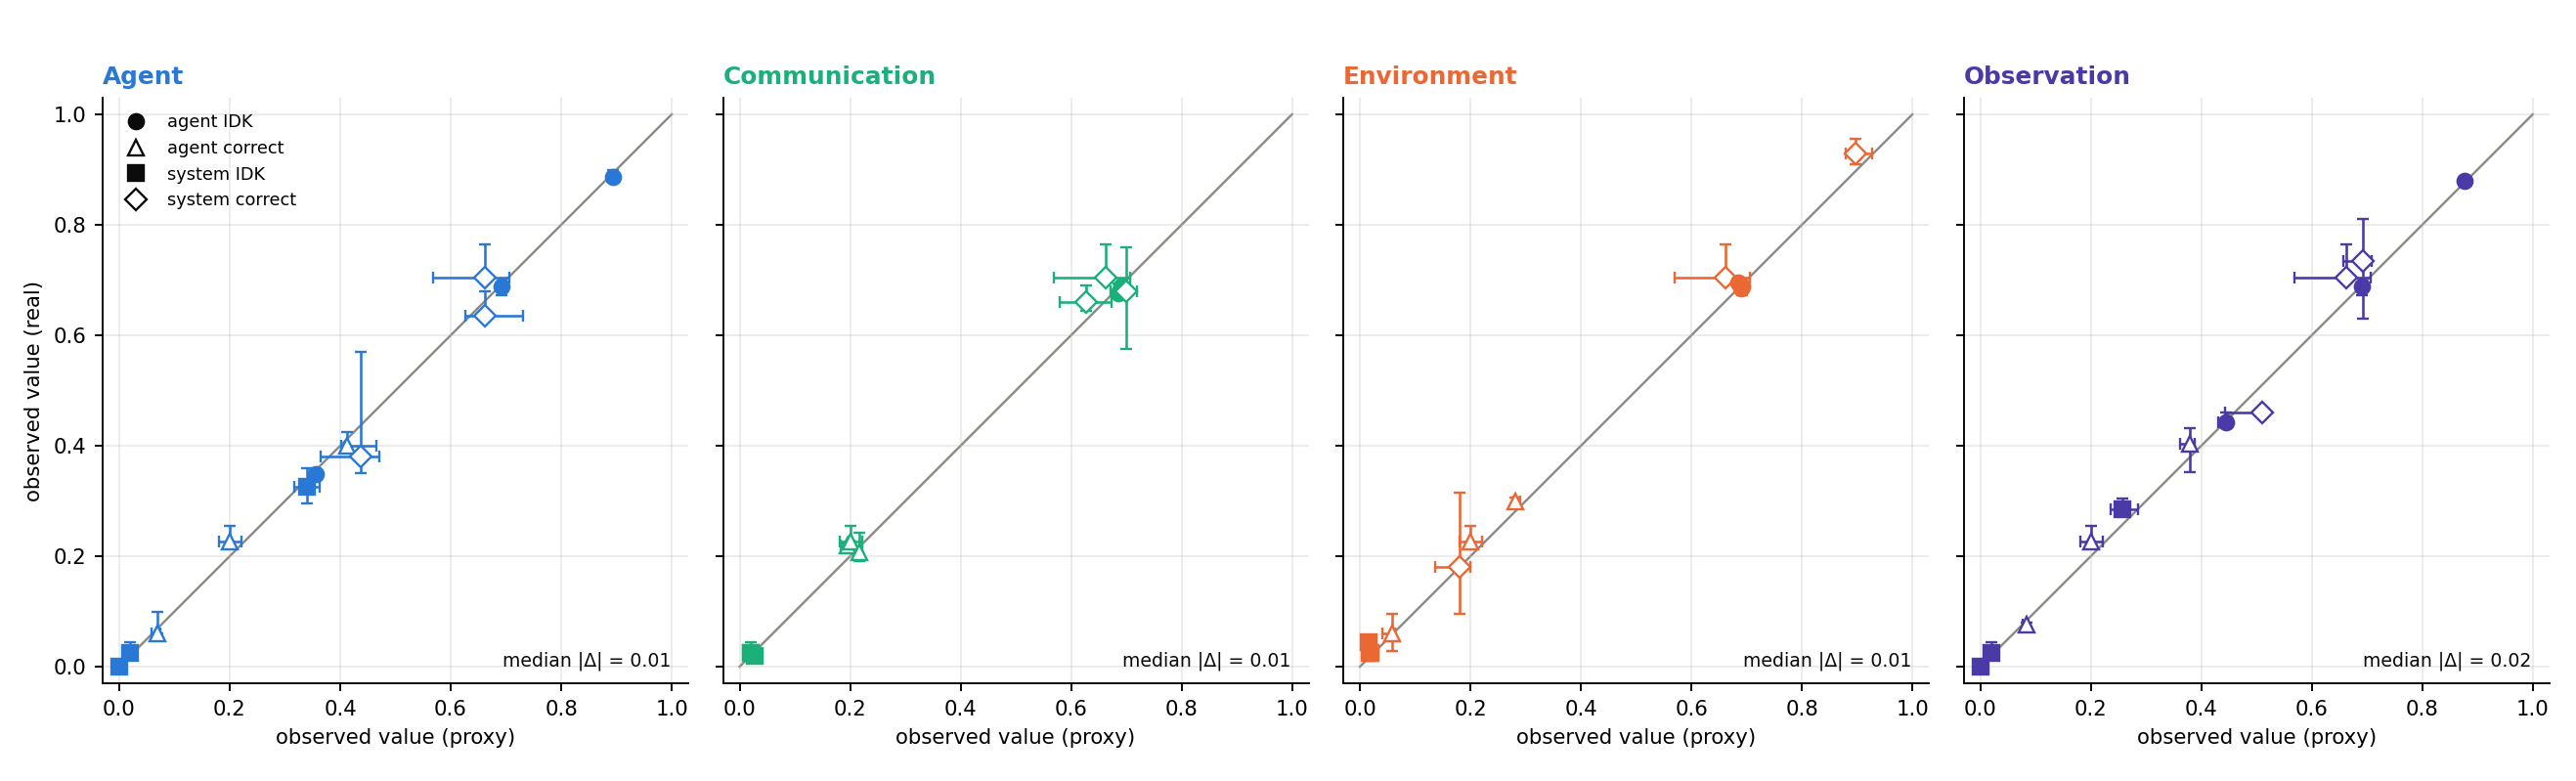
\includegraphics[width=0.98\textwidth]{figure2_paper.png}
  \caption{\textbf{Validation of the proxy: the simulation matches the real system, per factor, with zero fitted parameters.} Each panel: that factor's three settings $\times$ four metrics, plotted as simulation (horizontal, median with 10-seed IQR) against real (vertical, median with seed range). The chain is: measured answering gate $P(\text{response category}\mid\text{context state})$ + verbatim relay + mechanical retrieval. Median $|\Delta| = 0.01$ in every factor; the same holds for the mimesis grid (not shown).}
  \label{fig:cal}
\end{figure*}

\subsection{Epistemic collapse}
\label{sec:collapse}
We say an agent has \emph{epistemically collapsed} on a question set when it can no longer ground answers and produces only abstentions; the \emph{system} has collapsed when no member can answer. Collapse has a quieter twin: an agent whose evidence has expired but still surfaces it answers \emph{confidently and wrongly} --- availability survives, accuracy dies. Both matter, and every mechanism below prices them differently.

Figure~\ref{fig:example} shows a real system experiencing collapse, next to a healthy control identical in every respect except memory decay ($c=1.0$ vs.\ $c=0.05$). In perspective space --- each agent embedded by its probe responses, à la our earlier work --- the healthy agents move through the region of content-bearing answers, while the collapsing system's agents sit pinned to the ``I don't know'' point (left). The average member of the collapsing system abstains $\sim$90\% of the time and is correct $\sim$3\% of the time (middle, right). A factor-structured survey of the same real system (grid figures in the project artifacts) shows every factor owns a lever that carries the real system between health and collapse --- decay ($c: 0.05 \to 1.0$ takes agent IDK $0.35 \to 0.89$), observation starvation ($E: 6 \to 1$ takes system IDK $0 \to 0.29$), while environment speed ($\bar\lambda: 0.001 \to 0.1$) collapses \emph{accuracy} (system: $0.93 \to 0.20$) without moving abstention at all --- the confident-staleness regime. Degree is flat here by design: without secondhand information, the graph cannot matter.

The rest of this note studies the two natural \emph{mitigations}, both forms of communication: (1) \textbf{sharing secondhand information} (mimesis) --- letting agents repeat answers they received rather than observed; and (2) \textbf{books} --- a shared artifact agents write to and read from. Both run on the validated platform of Sec.~2.

\section{Mitigation 1: sharing secondhand information}
\label{sec:mimesis}
The mimesis grid repeats the factor design of Sec.~2 with one change: received answers may ground an answer (still verbatim --- agents repeat, they do not paraphrase). Figure~\ref{fig:policy} overlays the two grids at the agent level.

\textbf{Mimesis raises the floor.} At baseline, agent-level IDK drops $0.68 \to 0.26$ and agent accuracy rises $0.23 \to 0.48$. The communication factor switches from a null lever to a live one: agent accuracy is $0.38$ at degree 2 vs.\ $0.56$ on the mesh, where without mimesis the same sweep is flat.

\textbf{But not the ceiling.} System-level accuracy does not improve --- $0.72$ (no mimesis) vs.\ $0.66$ (mimesis) at baseline --- because the system level asks whether \emph{anyone} holds current evidence, and repetition redistributes evidence without creating it. Mimesis pays at the system level only where redistribution is the binding constraint: in the observation-starved cell ($E=1$) system accuracy rises $0.46 \to 0.64$ and system IDK falls $0.29 \to 0.02$. The regime it cannot rescue is fast forgetting ($c=1.0$: system IDK $0.33$ vs.\ $0.31$) --- copies crowd out as fast as originals.

\begin{figure*}[b]
  \centering
  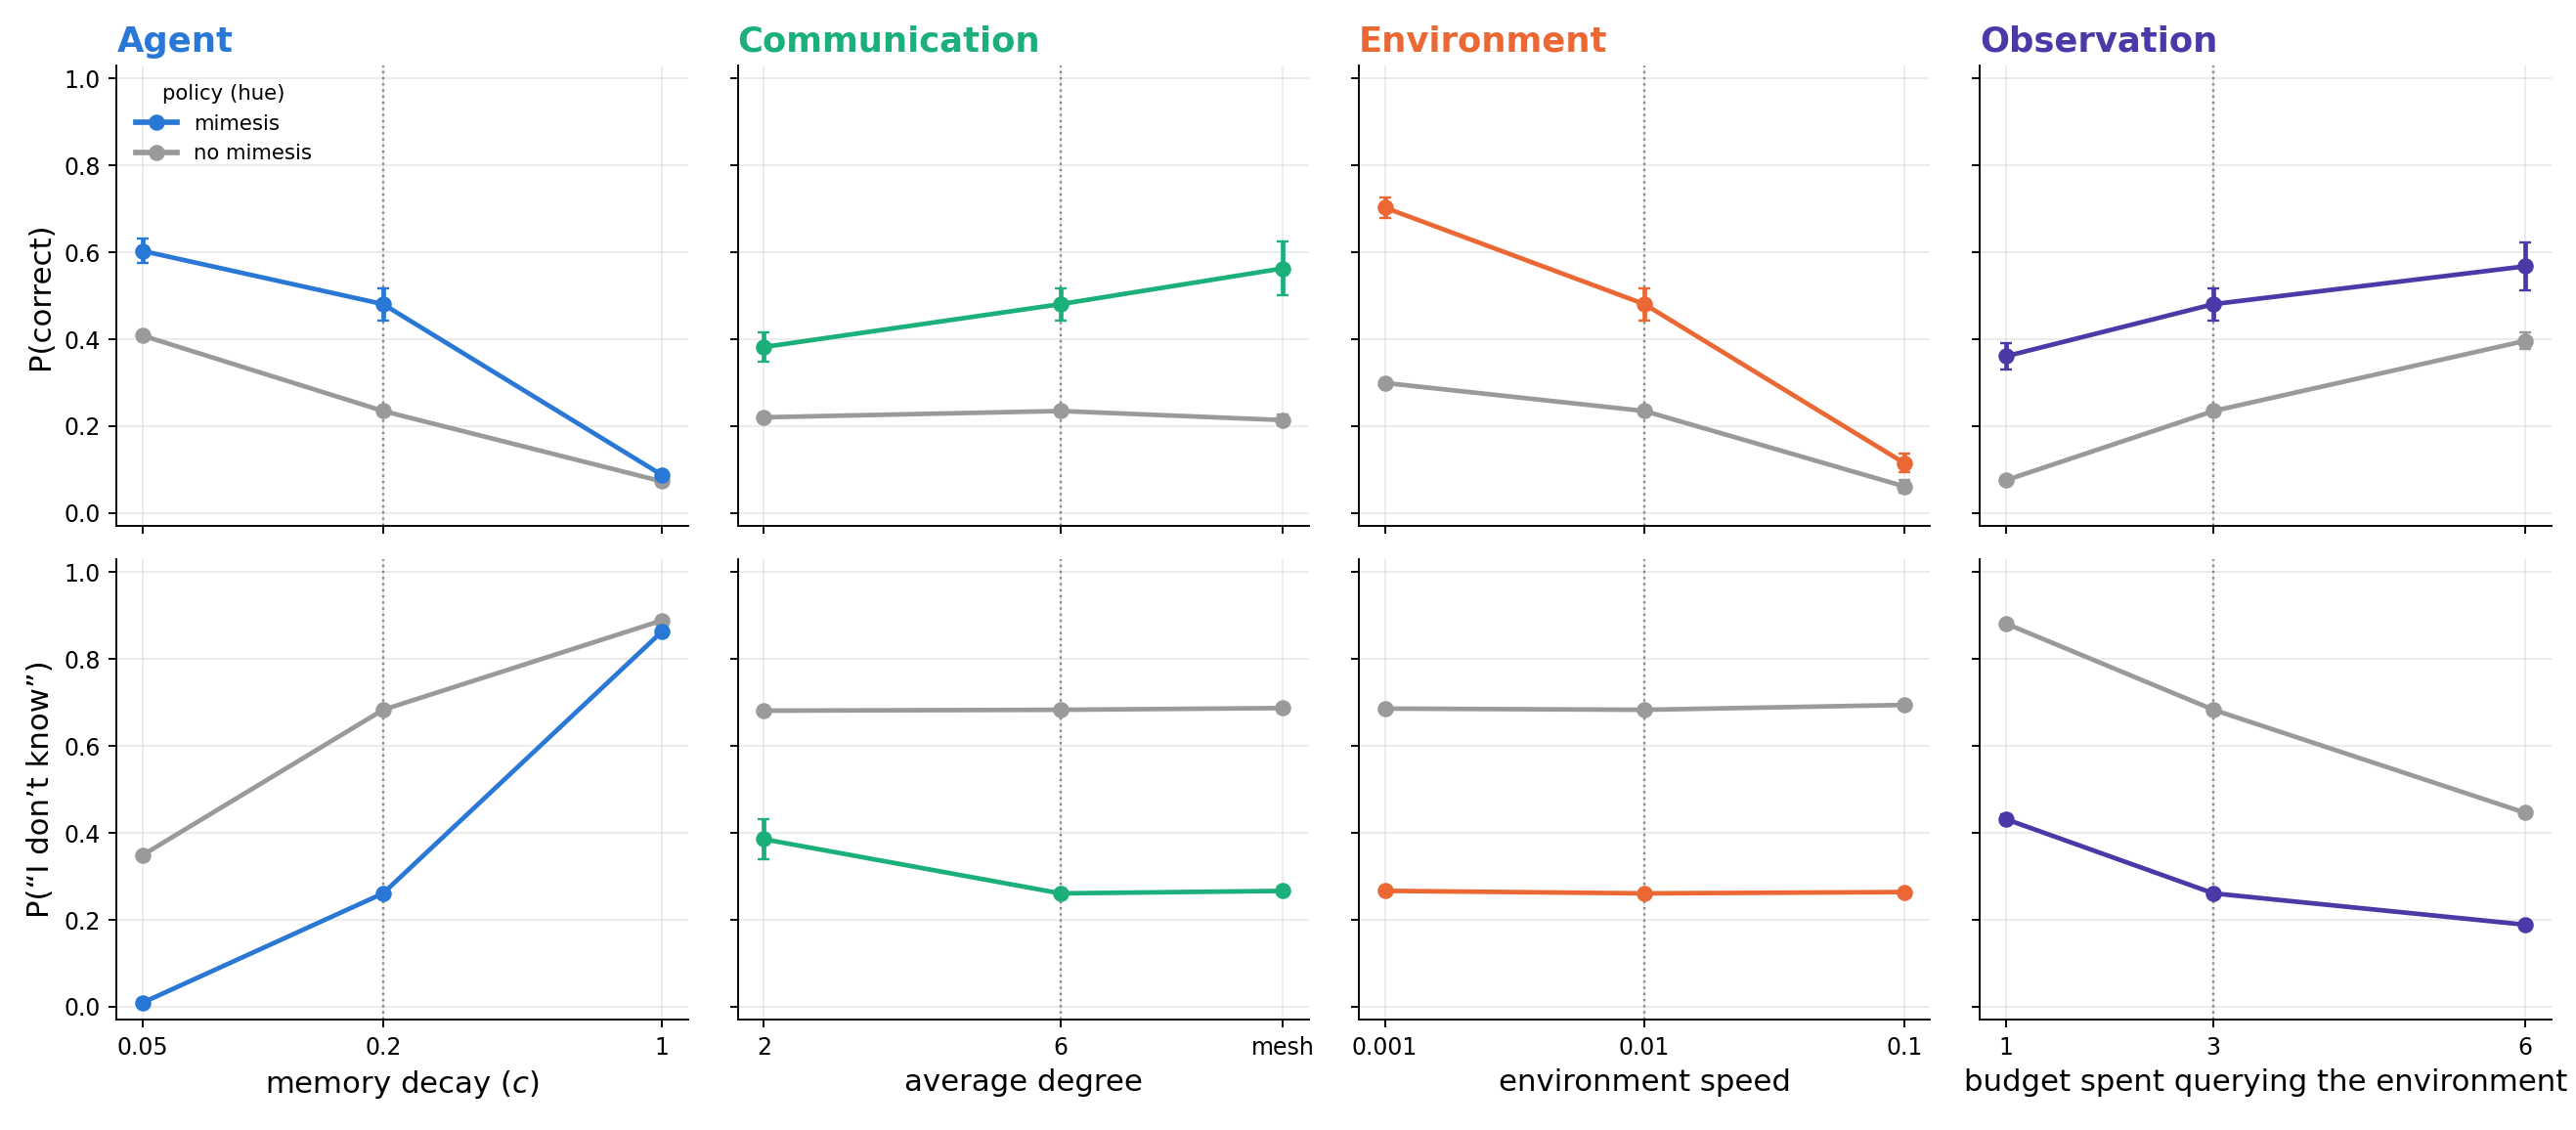
\includegraphics[width=0.95\textwidth]{figure_internal_policy_agentlevel.png}
  \caption{\textbf{Sharing secondhand information raises the floor, not the ceiling} (agent level; same factor grids and protocol as Sec.~2, mimesis vs.\ no mimesis overlaid). Mimesis roughly halves abstention and doubles accuracy for the average member at baseline and brings the communication graph into play; system-level accuracy (not shown) stays environment-capped: $0.72$ vs.\ $0.66$ at baseline.}
  \label{fig:policy}
\end{figure*}

\section{Mitigation 2: books}
Mimesis is peer-to-peer. The second mitigation is a shared artifact: a \emph{book} any agent can read for one action, fed only by deliberate, costly writes --- an agent attempts a write with probability $p$, an attempt consumes its entire step, and a write commits after $W$ attempts, merging the writer's current grounded knowledge (newest evidence wins). Reads ground answers like observations. We sweep the toy platform (10 seeds per point) in a scarce-observation regime where books have room to matter.

\textbf{The book's value is a race between its write rate and the world's revision rate.} The natural unit is the expected write rate $\omega = p/W$ (completed writes per agent per step). The book's accuracy gain over the no-books floor is large when $\bar\lambda \ll \omega$ ($+0.48$ at $\omega = 10/100$ steps, $\bar\lambda = 0.001$) and gone when $\bar\lambda/\omega \gtrsim 1$: every condition lands on the floor by $\bar\lambda = 0.3$ (Fig.~\ref{fig:books}, left). Availability behaves completely differently: P(IDK) is set by $\omega$ ($0.43/0.63/0.83$ for $\omega = 10, 1, 0.2$ per 100 steps, vs.\ $0.93$ without books) and is \emph{flat in $\bar\lambda$} (Fig.~\ref{fig:books}, right). Staleness absorbs the entire loss: the book keeps everyone answering while the answers quietly expire --- a fast world does not silence the library, it turns it into a confident source of expired facts.

\textbf{$\omega$ is the sufficient statistic.} Holding $p$ fixed and varying $W$ (constant budget tax) reproduces the ordering, confirming $W$ is a pure freshness dial with diminishing returns once the book turns over faster than the world. Conversely, holding $\omega$ fixed while varying $p$ by $4$--$10\times$ moves the curves by at most $0.06$ on either metric, against between-$\omega$ gaps up to $0.22$. The residual is monotone in $p$ with the sign a budget tax predicts (high-$p$ writers lose more steps to attempts and deposit slightly staler content, $\approx 0.04$--$0.06$ accuracy at slow speeds). For design purposes: quote a book policy by its expected writes; the attempt probability is a second-order tax.

\begin{figure*}[b!]
  \centering
  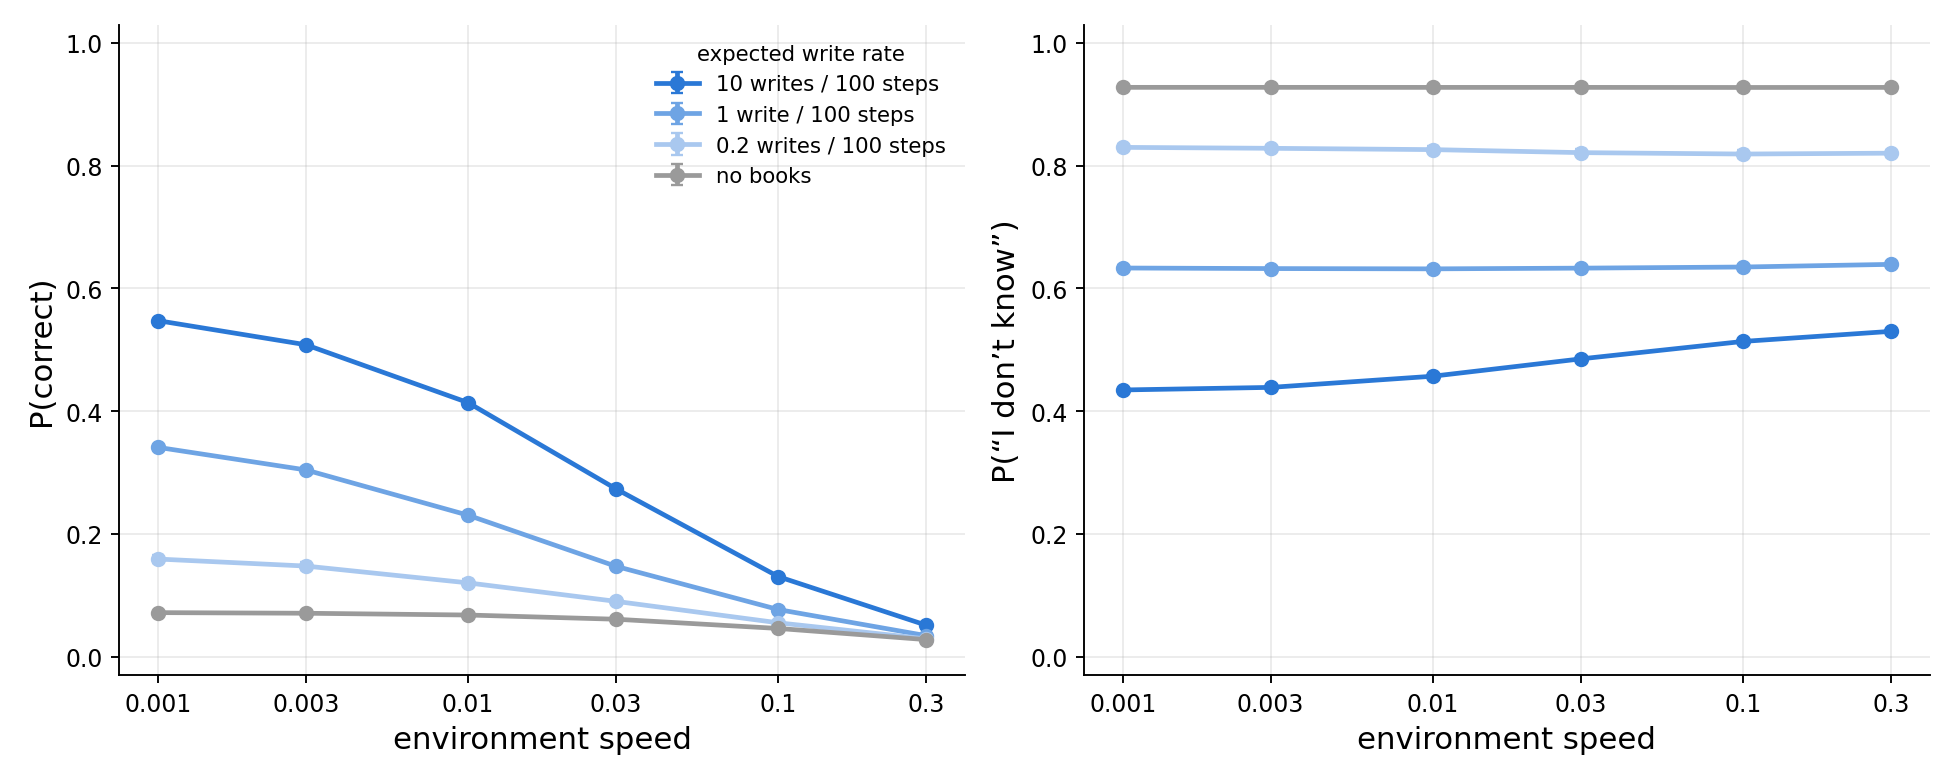
\includegraphics[width=0.82\textwidth]{fig_books_costly.png}
  \caption{\textbf{A book buys availability at any speed; its accuracy dies at $\bar\lambda/\omega \sim 1$.} Toy platform, no mimesis, scarce observation; conditions labeled by expected write rate $\omega = p/W$. Left: accuracy with the book converges to the no-books floor as $\bar\lambda$ rises, for every $\omega$. Right: P(IDK) is set by $\omega$ and essentially flat in $\bar\lambda$.}
  \label{fig:books}
\end{figure*}

\paragraph{Takeaway and next steps.} Communication --- secondhand sharing or shared artifacts --- reliably buys \emph{availability}, and buys \emph{accuracy} only while the underlying evidence is younger than the world's revision clock: mimesis is capped by what the population has observed, and a book by how often anyone can afford to write. As the environment speeds up, the failure mode is not silence but confident staleness, which availability metrics cannot see. Next: (1) ``dated editions'' --- books exposing their write time so readers can abstain on stale entries, trading availability back for accuracy; (2) strategy-sensitivity sweeps on the validated platform; (3) the monitoring question: does a control chart on the probe panel see confident staleness coming, given it presents as drift, not shift?

\end{document}
